\documentclass{beamer}
\usepackage[utf8]{inputenc}
\usepackage{caption}
\usepackage{subcaption}
\usepackage{tabularx}

\newenvironment{changemargin}[2]{%
  \begin{list}{}{%
    \setlength{\topsep}{0pt}%
    \setlength{\leftmargin}{#1}%
    \setlength{\rightmargin}{#2}%
    \setlength{\listparindent}{\parindent}%
    \setlength{\itemindent}{\parindent}%
    \setlength{\parsep}{\parskip}%
  }%
  \item[]}{\end{list}}

\usetheme{Darmstadt}

\title{Animat}
\subtitle{Using coloured snapshots for short-range guidance in mobile robots \cite{Gourichon2002}}
\author{Paul Moncuquet \& Thibaut Munzer}

\begin{document}

\begin{frame}
  \titlepage
\end{frame}

\begin{frame}
  \frametitle{Sommaire}
  \tableofcontents%[pausesections]
\end{frame}

\section{Introduction}

\subsection{Problématique}

\begin{frame}
  \frametitle{Problématique}
  \begin{block}{\textit{Homming}}
  \begin{itemize}
    \item \textit{Snapshot} de l'objectif
    \item Près de l'objectif
    \item Utilisation de données visuelles
    \item Méthode basée sur la mise en correspondance d'amers (\textit{matching})   
  \end{itemize}
  \end{block}

  \begin{block}{Approche Animat}
  \begin{itemize}
    \item Transposition du comportement des abeilles dans un contexte robotique
    \item Par exemple pour le retour à la base d'alimentation
  \end{itemize}
  \end{block}
\end{frame}

\subsection{Travaux existants}

\begin{frame}
  \begin{block}{Modèle Cartwright \& Collett \cite{Carwright1983}}
    \begin{itemize}
      \item Inspiré des abeille
      \item Hypothèse d'orientation connue
      \item Création d'un pannoramma
      \item \textit{Matching} au plus proche (dans le \textit{snapshot})
      \item Calcul des composantes tangentielles et radiales    
      \begin{figure}
        \centering
        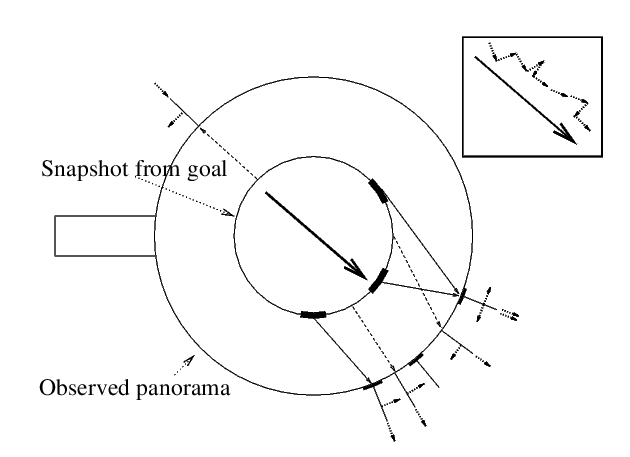
\includegraphics[scale=0.2]{cc_model.png}
        \caption{Modèle CC}
      \end{figure}
    \end{itemize}
  \end{block}
\end{frame}

\begin{frame}
  \begin{block}{Modèle PV}
    \begin{itemize}
      \item Proposé par Möller et al. \cite{Lambrinos2000}
      \item Contribution de chaque vecteur proportionelle à la différence lors du \textit{matching}
    \end{itemize}
  \end{block}
  \begin{block}{Modèle Gourichon}
    \begin{itemize}
      \item Modèle de l'article étudié
      \item Basé sur le PV modèle
      \item Hypothèse d'orientation fixe
      \item Angle de vue limité ($220^{\circ}$)
      \item Amélioration du matching
      \item Utilisation de la couleur 
      \item Suppression de la composante radiale
    \end{itemize}
  \end{block}
\end{frame}

\section{Matériels, méthodes et résultats}

\subsection{Reproduction des résultats}

\begin{frame}
  Deux expériences dans l'article :
  \begin{itemize}
    \item Une expérience virtuelle
    \begin{figure}
      \centering
      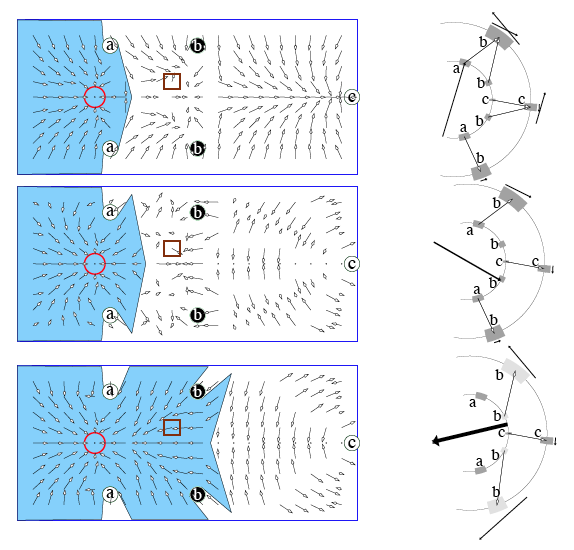
\includegraphics[scale=0.2]{Exp-virtuel.png}
    \end{figure}
    \item Une expérience réelle
    \begin{figure}
      \centering
      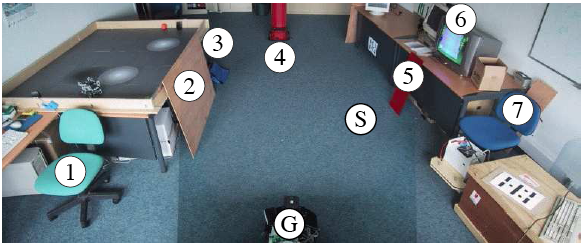
\includegraphics[scale=0.2]{Exp-real.png}
    \end{figure}
  \end{itemize}
  Reproduction de l'éxpérience virtuelle
\end{frame}

\begin{frame}
  \begin{block}{Mise en place d'un simulateur}
    \begin{itemize}
      \item Choix de ne pas utiliser un simulateur existant
      \item Utilisation de SDL
    \end{itemize}
  \end{block}
  \begin{figure}
    \centering
    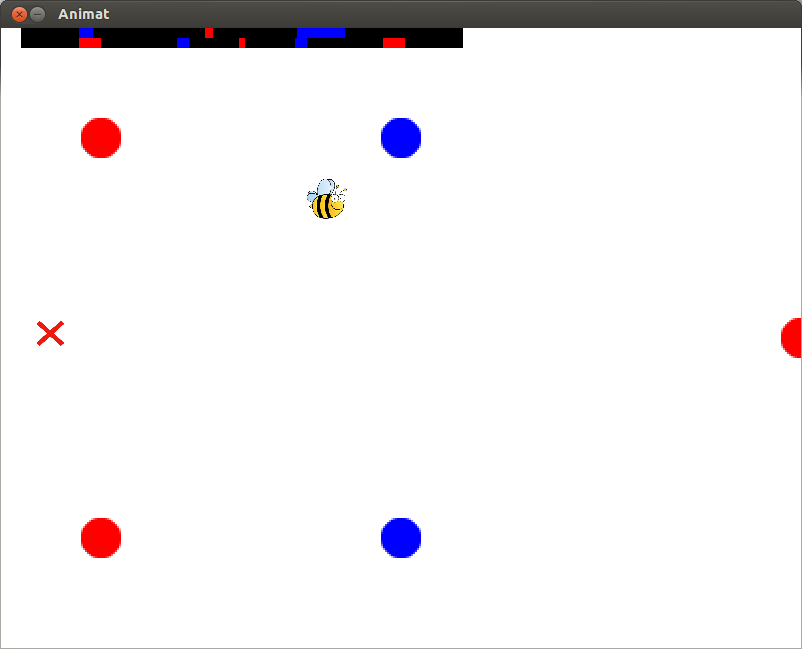
\includegraphics[scale=0.2]{one_run.png}
    \caption{Exemple simulateur}
  \end{figure}
\end{frame}

\begin{frame}
  \begin{block}{Calcul de la zone de convergence}
    \begin{itemize}
      \item Discrétisation du monde
      \item Problème du cas d'arret
      \item Optimisation du calcul
    \end{itemize}
  \end{block}
  \begin{figure}
    \centering
    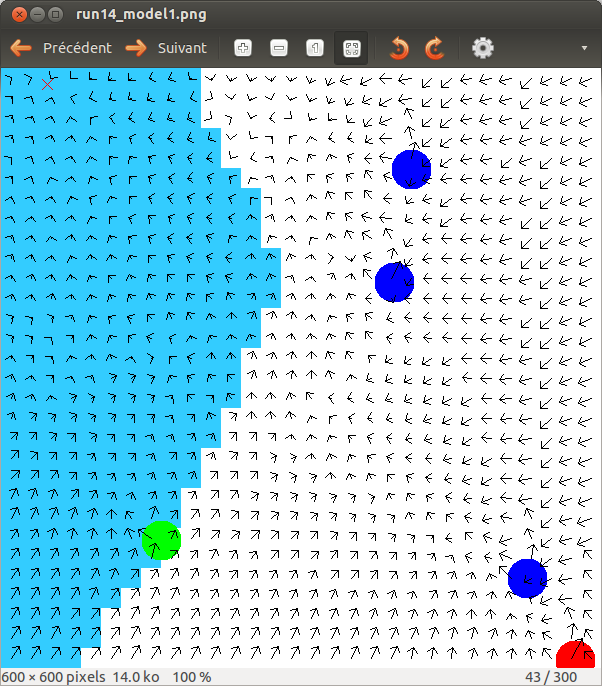
\includegraphics[scale=0.2]{exp.png}
    \caption{Exemple zone de convergence}
  \end{figure}
\end{frame}

\subsection{Comparaison des résultat}

\begin{frame}
  \frametitle{Modèle PV}
  \begin{figure}
    \centering
    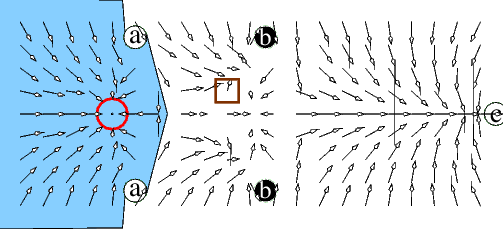
\includegraphics[scale=0.3]{pv_article.png}
  \end{figure}
  \begin{figure}
    \centering
    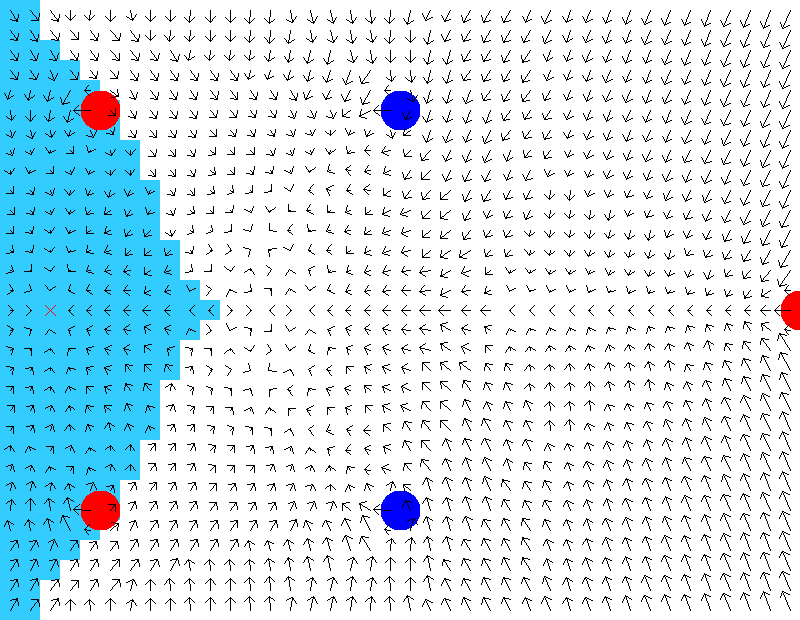
\includegraphics[scale=0.15]{pv1_res.png}
    \caption{Comparaison modèle PV}
  \end{figure}  
\end{frame}

\begin{frame}
  \frametitle{Modèle PV : Contributions modifiées}
  \begin{figure}
    \centering
    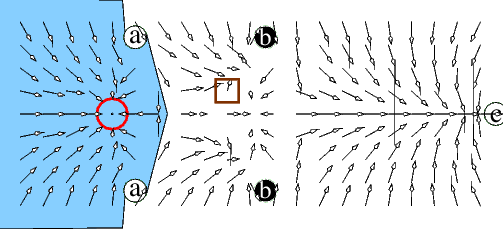
\includegraphics[scale=0.3]{pv_article.png}
  \end{figure}
  \begin{figure}
    \centering
    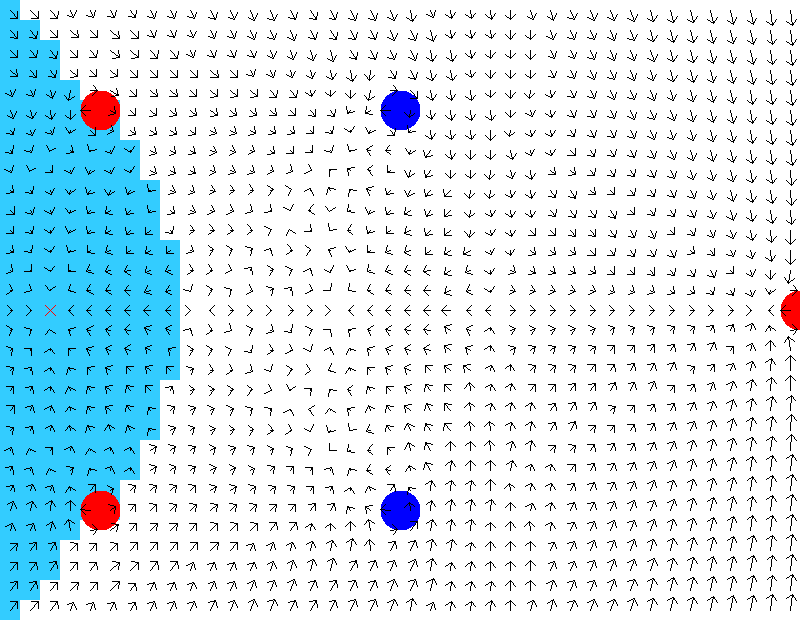
\includegraphics[scale=0.15]{pv2_res.png}
    \caption{Comparaison modèle PV}
  \end{figure}  
\end{frame}

\begin{frame}
  \frametitle{Modèle Gourichon sans couleur}
  \begin{figure}
    \centering
    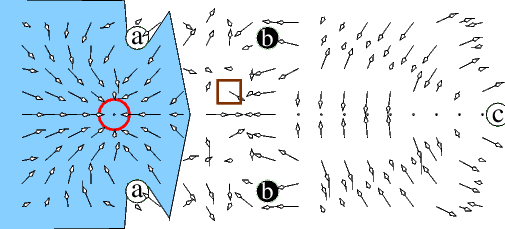
\includegraphics[scale=0.3]{nocolor_article.png}
  \end{figure}
  \begin{figure}
    \centering
    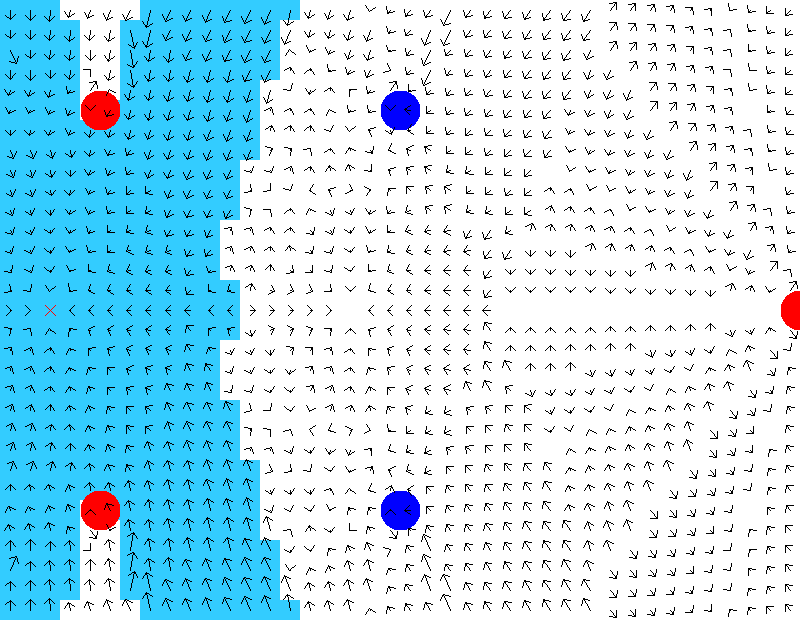
\includegraphics[scale=0.15]{nocolor_res.png}
    \caption{Comparaison modèle Gourichon sans couleur}
  \end{figure}  
\end{frame}

\begin{frame}
  \frametitle{Modèle Gournichon}
  \begin{figure}
    \centering
    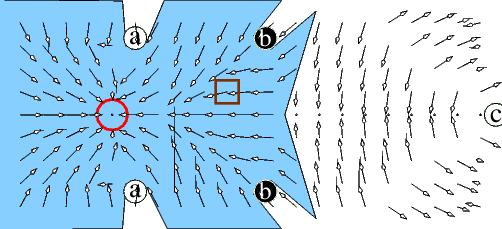
\includegraphics[scale=0.3]{color_article.png}
  \end{figure}
  \begin{figure}
    \centering
    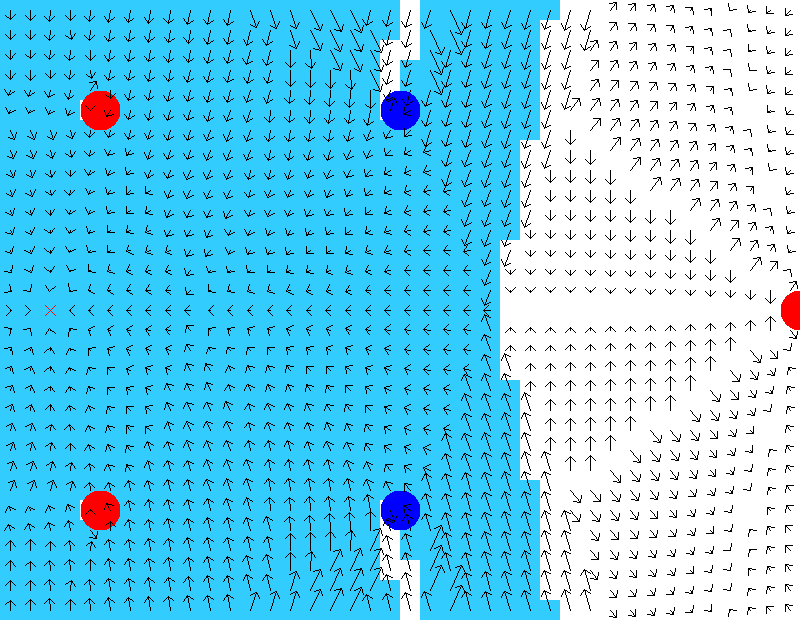
\includegraphics[scale=0.15]{color_res.png}
    \caption{Comparaison modèle Gournichon}
  \end{figure}  
\end{frame}

\section{Discussion et conclusion}

\subsection{Discussion}

\begin{frame}
  \frametitle{Etude des performances sur un grand nombre de scènes}
  \begin{changemargin}{-1.0cm}{0cm}
  \begin{figure}
    \centering
    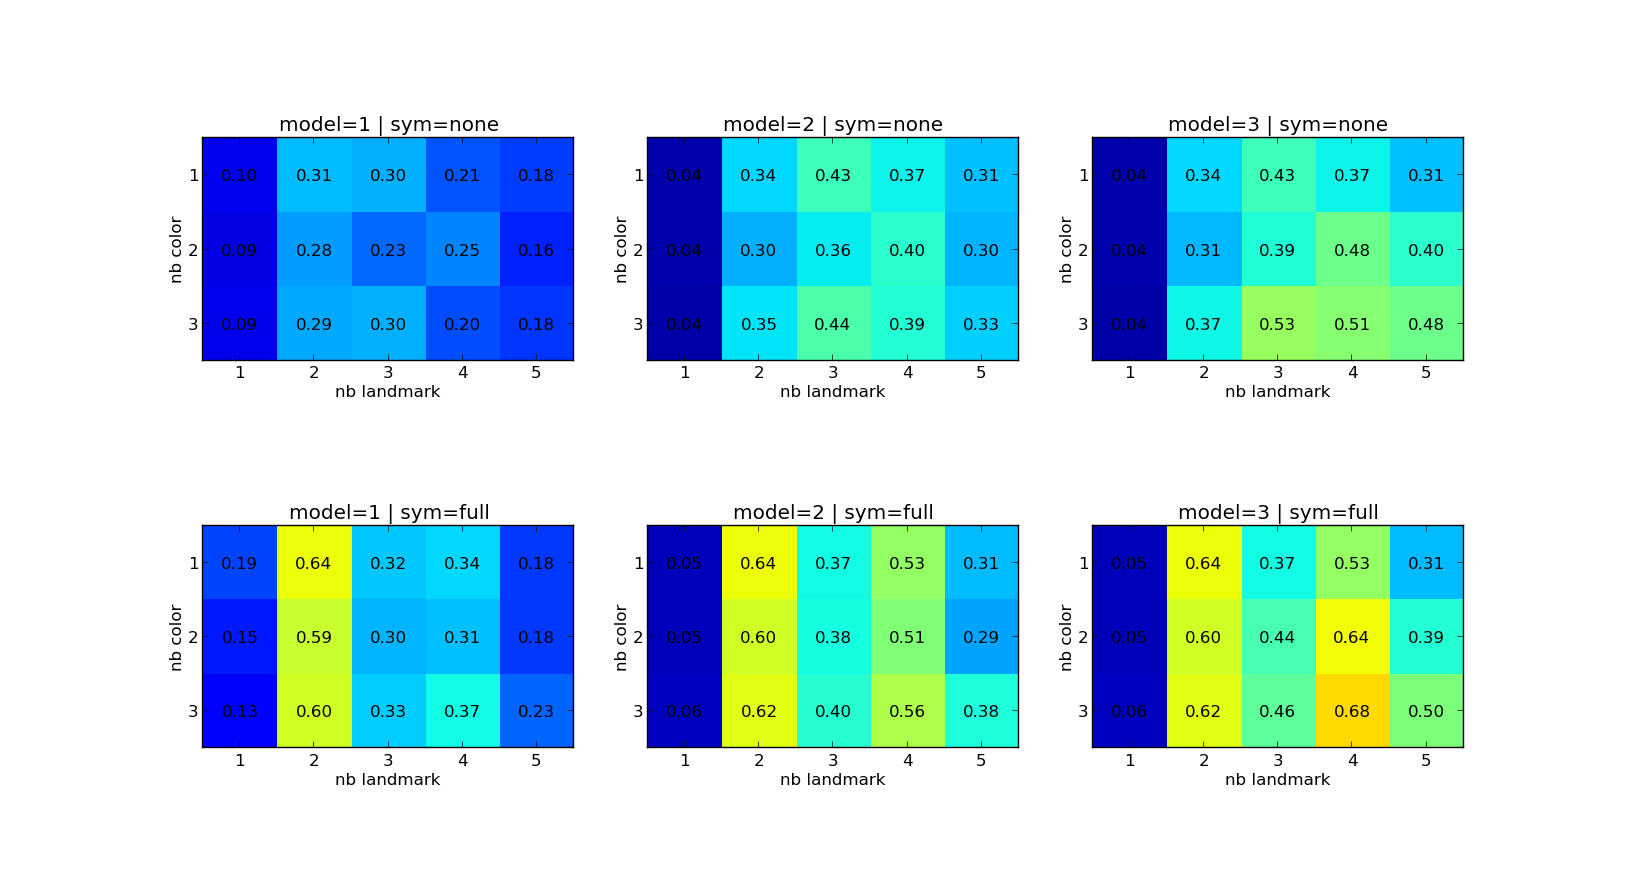
\includegraphics[scale=0.3]{res_sym.png}
  \end{figure}  
  \end{changemargin}
\end{frame}

\begin{frame}
  \frametitle{Etude des performances en ajoutant la composante radiale}
  \begin{changemargin}{-1.0cm}{0cm}
  \begin{figure}
    \centering
    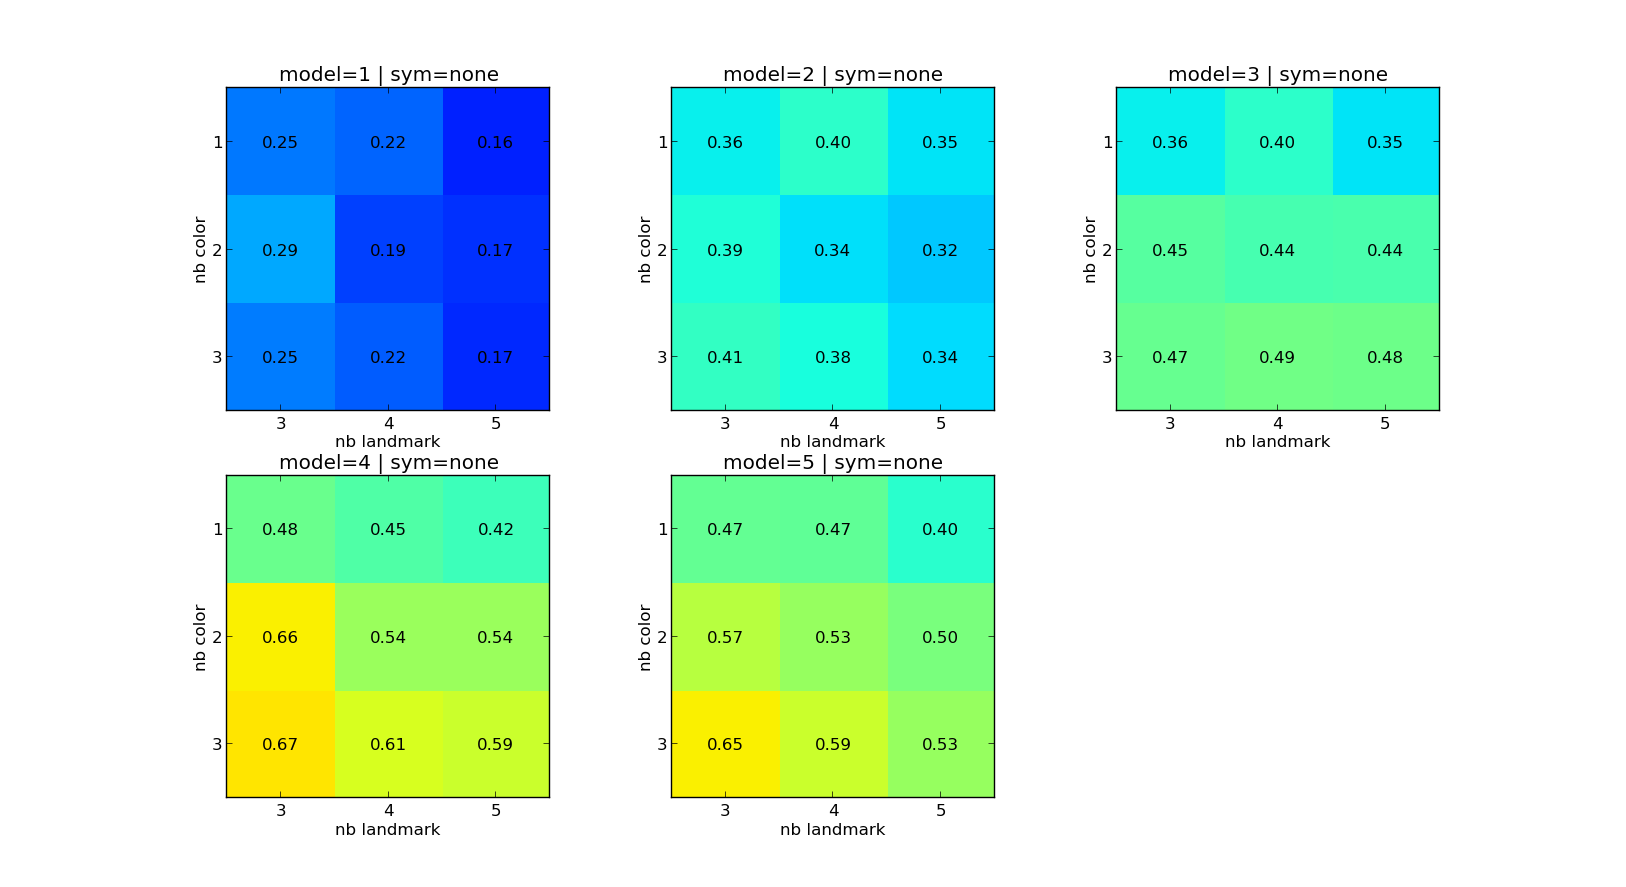
\includegraphics[scale=0.3]{res_45.png}
  \end{figure}  
  \end{changemargin}
\end{frame}

\subsection{Conclusion}% Conclusion

\begin{frame}
  \frametitle{Conclusion}
  \begin{block}{Retour sur expérience}
    \begin{itemize}
      \item Lecture et compréhension d'un article
      \item Reproduction des résultats
      \item Amélioration du processus de validation du modèle proposé
      \item Réintégration de la composante radial et amélioration des résultats    
    \end{itemize}
  \end{block}
  \begin{block}{Ouverture}
    \begin{itemize}
      \item Relacher la contrainte d'orientation
      \item Utilisation de données visuelles en deux dimmensions
    \end{itemize}
  \end{block}
\end{frame}

\begin{frame}{Références}
  \nocite{*}
  \bibliographystyle{plain}
  \bibliography{Animat.bib}
\end{frame}

\end{document}